\documentclass[11pt,a4paper]{article}
\usepackage[english]{babel}
\usepackage[a4paper,margin=1in]{geometry}
\usepackage[T1]{fontenc}
\usepackage{lmodern}
\usepackage{microtype}
\usepackage{amsmath,amssymb,graphicx}
\usepackage[hidelinks]{hyperref}
\usepackage[font=small,skip=4pt]{caption}
\usepackage{enumitem}
\graphicspath{{figures/}}
\setlength{\parskip}{4pt}
\setlength{\parindent}{0pt}
\title{Understanding Neural Ordinary Differential Equations\\\large From Exponential Decay to Epidemic Models}
\author{Veronika Rybak\\Bachelor Seminar\\Supervisor: Prof.\ Dr.\ Nadja Ray}
\date{\today}

\begin{document}
\maketitle

\begin{abstract}
Neural Ordinary Differential Equations (Neural ODEs) combine a neural network
with an ordinary differential equation solver. The network does not directly
predict a complete time series. It gives a rule for the current rate of change,
and the solver repeatedly uses this rule to construct a trajectory. This report
explains the idea through four small, reproducible experiments: Euler
approximation, learning a decay rate, learning a decay rule with a neural
network, and a two-dimensional susceptible--infected (SI) epidemic model. The
experiments show both what can be learned from observations and why conclusions
must be limited to the states represented by the training data. The final
section connects these examples to the graph-based epidemic model of Kosma et
al.\ \cite{kosma2023}.
\end{abstract}

\tableofcontents
\newpage

\section{Introduction}

An ordinary differential equation (ODE) describes how a quantity changes. A
Neural ODE uses the same idea, but represents the rule of change by a neural
network. It is important to separate three objects:
\[
\text{current state}\quad\longrightarrow\quad
\text{rule of change}\quad\longrightarrow\quad
\text{trajectory}.
\]
The state is the current value of a system. The rule gives its derivative at
that value. A numerical solver turns many local derivatives into a trajectory.

This report asks three simple questions:
\begin{enumerate}[label=\arabic*.]
\item How does an ODE turn a local rule into a curve?
\item How can observations be used to learn that rule?
\item Can the same learned rule be used from a different starting point?
\end{enumerate}
The examples begin with systems that can be checked exactly. Exponential decay
has one state variable. The SI model has two state variables and an interaction
between them. Only after these basic examples do we move to epidemic spreading
on a contact network.

\section{ODE foundations}

\subsection{A rule of change and an initial value}

A first-order ODE has the form
\begin{equation}
\frac{dy(t)}{dt}=f(y(t),t).
\label{eq:ode}
\end{equation}
The unknown is a function $y(t)$, not one number. The function $f$ gives the
instantaneous rate of change. To select one particular curve, an initial value
is required:
\begin{equation}
y(t_0)=y_0.
\label{eq:initial}
\end{equation}
Together, these form an initial value problem. The ODE says how the system
moves; the initial value says where the motion begins.

\subsection{Exponential decay}

The running example is exponential decay,
\begin{equation}
\frac{dy}{dt}=-\lambda y,\qquad y(0)=y_0,\qquad\lambda>0.
\label{eq:decay}
\end{equation}
The amount decreases at a rate proportional to its current value. Its exact
solution is
\begin{equation}
y(t)=y_0e^{-\lambda t}.
\label{eq:decay_solution}
\end{equation}
This exact solution lets us check a numerical method.

\subsection{Experiment 1: building a curve with Euler's method}

Many ODEs have no exact solution that is easy to use. Forward Euler is the
simplest numerical method:
\begin{equation}
y_{n+1}=y_n+h f(y_n,t_n),
\label{eq:euler}
\end{equation}
where $h$ is the step size. It evaluates the derivative at the current point
and takes a short step in that direction.

For \eqref{eq:decay} with $\lambda=0.8$, $y_0=1$, and $h=0.5$, the first step is
\[
y_1=1+0.5(-0.8\cdot1)=0.6.
\]
Repeating this calculation creates an approximation to the curve.
Figure~\ref{fig:euler} compares the exact curve on $[0,5]$ with two Euler
approximations. The maximum error is $0.089$ for $h=0.5$ and $0.0075$ for
$h=0.05$. Smaller steps use more calculations but follow the exact curve more
closely.

\begin{figure}[ht]
\centering
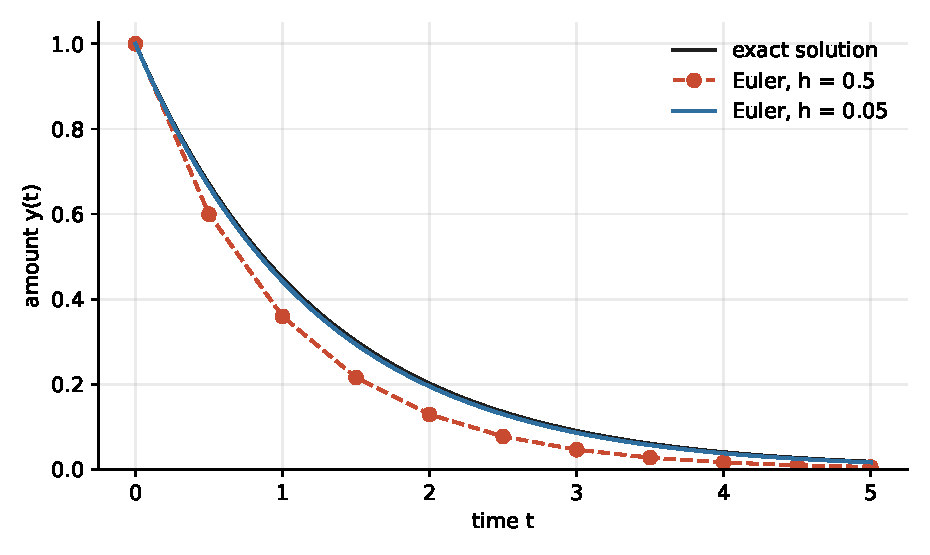
\includegraphics[width=.78\textwidth]{01_euler_decay.pdf}
\caption{Experiment 1: Euler approximations to $y'=-0.8y$, $y(0)=1$.}
\label{fig:euler}
\end{figure}

The solver has this same role in every later experiment. It does not learn from
data; it only follows the rule supplied to it.

\section{Learning a differential equation}

\subsection{The Neural ODE idea}

A Neural ODE replaces a known rule $f$ by a trainable function $f_\theta$:
\begin{equation}
\frac{dh(t)}{dt}=f_\theta(h(t),t).
\label{eq:neural_ode}
\end{equation}
The parameters $\theta$ can change during training. Given an initial state, a
solver produces a predicted trajectory. At observation times $t_k$, it can be
compared with data $y^*(t_k)$ using mean squared error:
\begin{equation}
L(\theta)=\frac{1}{K}\sum_{k=1}^K
\bigl(y_\theta(t_k)-y^*(t_k)\bigr)^2.
\label{eq:loss}
\end{equation}

Training repeats four steps: solve the ODE with the current rule, compare the
prediction with observations, compute how the loss depends on $\theta$, and
update $\theta$. The update changes the rule of change, not an already
calculated trajectory.

\subsection{Experiment 2: recovering a decay rate}

\paragraph{Question.} If the form of the decay equation is known but its rate
is not, can observations recover that rate?

\paragraph{Setup.} Reference observations were generated with
$\lambda=0.8$, $y_0=1$, at times $0,0.5,\ldots,5$. The model used
$f_\theta(y)=-\theta y$, began at $\theta=0.3$, and was solved by Euler's method
with $h=0.01$. Adam optimization with learning rate $0.001$ ran for 2,000
updates.

\paragraph{Result.} Figure~\ref{fig:parameter} shows an initially slow
prediction and a close fitted trajectory. The learned rate is $\theta=0.786$,
and the final mean squared error is $9.9\cdot10^{-6}$.

\begin{figure}[ht]
\centering
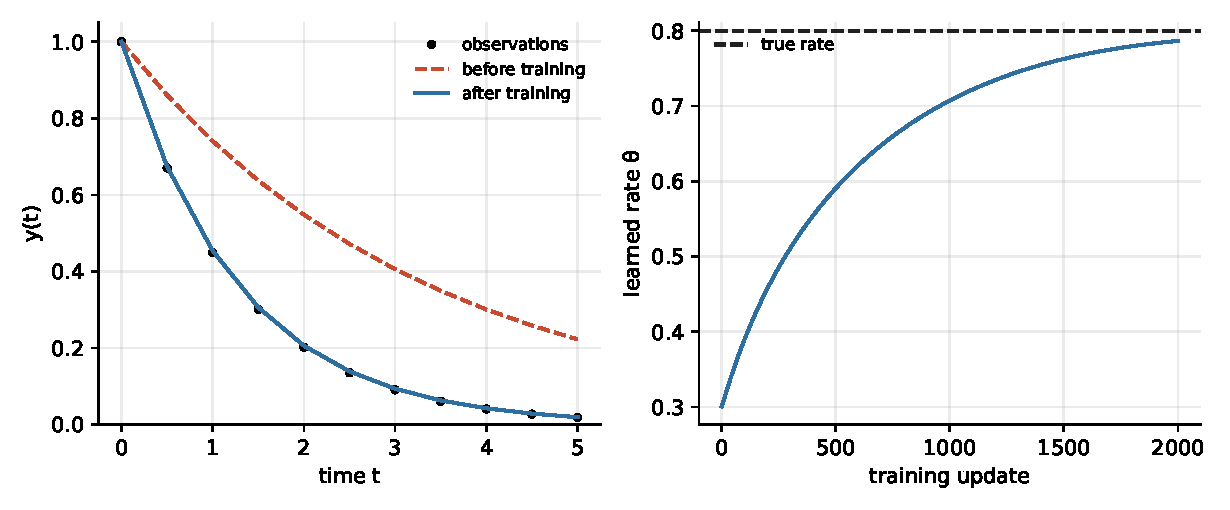
\includegraphics[width=.98\textwidth]{02_decay_parameter_learning.pdf}
\caption{Experiment 2: learning an unknown decay rate.}
\label{fig:parameter}
\end{figure}

This is parameter identification, not full function learning: the form
$-\theta y$ was supplied by the model.

\subsection{A small gradient calculation}

For one Euler step with $y_0=1$, step size $h$, and rule
$f_\theta(y)=-\theta y$, we have $y_1=1-h\theta$. If the observed value is
$y_1^*$ and $L(\theta)=(y_1-y_1^*)^2$, then the chain rule gives
\[
\frac{\partial L}{\partial\theta}
=2(y_1-y_1^*)\frac{\partial y_1}{\partial\theta}
=-2h(y_1-y_1^*).
\]
For many Euler steps, the same calculation is applied repeatedly. PyTorch's
automatic differentiation performs this bookkeeping in the experiments. A
small code test compares the automatic gradient with a finite-difference
approximation for one Euler step.

\subsection{Experiment 3: learning the decay rule with a neural network}

\paragraph{Question.} Can a neural network learn the rule of change when it
is not told that the rule should be a multiple of $y$?

\paragraph{Setup.} The observations are the same as in Experiment~2. This
time $f_\theta$ is a neural network with one input, one hidden layer of 16 tanh
units, and one linear output. It receives the current value $y$ and returns a
proposed derivative. The true derivatives $-0.8y$ are not training labels.

\paragraph{Result.} The left panel of Figure~\ref{fig:neural_decay} shows a
close fitted trajectory. Its final loss is $1.0\cdot10^{-5}$. The right panel
compares the learned rule with $-0.8y$ over the values visited by the
trajectory. Their mean squared difference there is $2.2\cdot10^{-4}$.

\begin{figure}[ht]
\centering
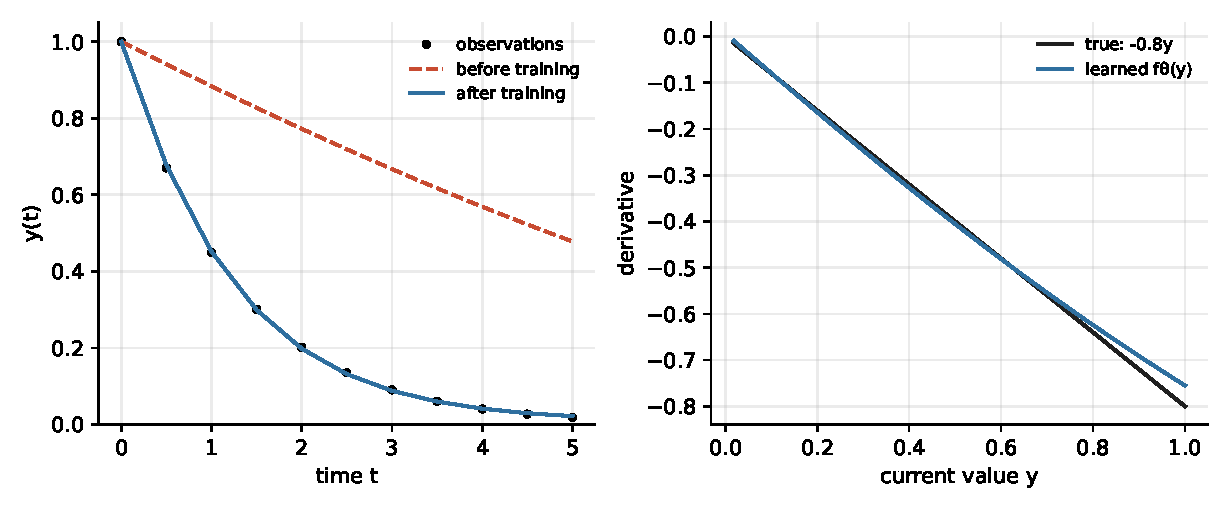
\includegraphics[width=.98\textwidth]{03_decay_neural_rule.pdf}
\caption{Experiment 3: a network learns a decay rule. Derivatives are used
only for the final comparison, not for training.}
\label{fig:neural_decay}
\end{figure}

The loss was computed from states along a curve, but the network represents
local derivatives. The result supports the learned rule only in the observed
range of $y$, not far outside it.

\section{From decay to the SI epidemic model}

\subsection{The SI equations}

The susceptible--infected (SI) model has two state variables: susceptible
fraction $S(t)$ and infected fraction $I(t)$. Once infected, an individual
stays infected:
\begin{align}
\frac{dS}{dt}&=-\beta SI,\\
\frac{dI}{dt}&=\beta SI.
\label{eq:si}
\end{align}
The product $SI$ represents encounters between susceptible and infected
individuals. Adding the equations gives $d(S+I)/dt=0$, so a population that
starts with $S+I=1$ stays normalized.

Because $S=1-I$, the second equation becomes
\[
\frac{dI}{dt}=\beta I(1-I).
\]
For initial infected fraction $I_0$, its exact solution is
\begin{equation}
I(t)=\frac{1}{1+\frac{1-I_0}{I_0}e^{-\beta t}},
\qquad S(t)=1-I(t).
\label{eq:si_solution}
\end{equation}
This logistic curve generates the reference observations.

\subsection{Experiment 4: a two-dimensional learned rule}

\paragraph{Question.} Does the same Neural ODE construction work when two
quantities change together?

\paragraph{Setup.} Reference data were generated from the SI equations with
$\beta=1$ on $[0,15]$. Two training trajectories started at $I_0=0.01$ and
$I_0=0.10$. A neural network with input $(S,I)$, one hidden layer of 16 tanh
units, and output $(\dot S,\dot I)$ was trained from the trajectories. It used
Euler's method with $h=0.2$, Adam with learning rate $0.001$, and 500 updates.
The coarser step makes the complete training calculation practical on an
ordinary CPU; this is a teaching demonstration, not a solver-accuracy study.

\paragraph{Result.} Figure~\ref{fig:si} compares learned and true derivatives
on the physical line $S=1-I$. It also solves the learned rule from
$I_0=0.05$, a starting point not used for training. The trajectory root mean
squared error is $0.114$, and the derivative mean squared error on the
physical line is $0.0106$. The prediction follows the general epidemic trend
but does not match the exact curve perfectly.

\begin{figure}[ht]
\centering
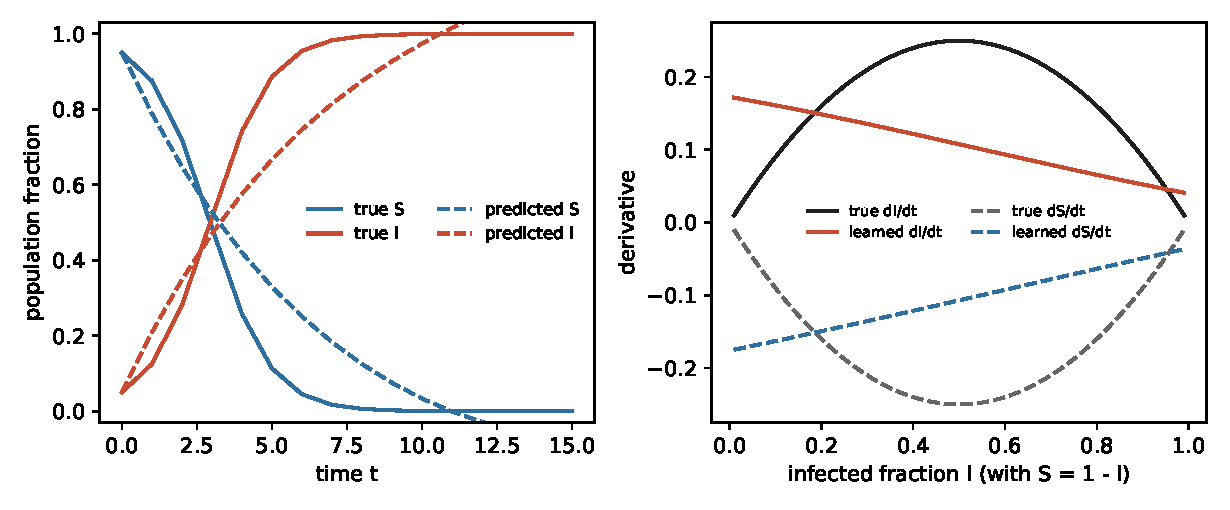
\includegraphics[width=.98\textwidth]{04_si_neural_rule_and_new_initial_condition.pdf}
\caption{Experiment 4: a learned SI rule. Left: prediction from the unseen
starting point $I_0=0.05$. Right: learned and true derivatives on $S=1-I$.}
\label{fig:si}
\end{figure}

The input and output of a learned rule can be vectors; the training procedure
does not otherwise change. However, all SI data here lie on the
one-dimensional line $S+I=1$. The new starting point is also on this familiar
line and between the two training conditions. It is an interpolation test, not
evidence that the network learned every possible two-dimensional state.

\section{From SI to SIR and network epidemics}

\subsection{Adding recovery}

The susceptible--infected--recovered (SIR) model adds a recovered fraction
$R(t)$ and recovery rate $\gamma$:
\begin{align}
\frac{dS}{dt}&=-\beta SI,\\
\frac{dI}{dt}&=\beta SI-\gamma I,\\
\frac{dR}{dt}&=\gamma I.
\end{align}
Thus $S+I+R=1$. The move from SI to SIR adds one state and one process:
infected individuals can recover.

\subsection{Network SIR and GN-ODE}

A well-mixed model treats every individual alike. A contact network represents
people by nodes and possible contacts by edges. Its adjacency matrix $A$
records which nodes can influence each other. For node-level probability
vectors $\mathbf{s}$, $\mathbf{i}$, and $\mathbf{r}$, a simple approximation is
\[
\frac{d}{dt}
\begin{pmatrix}\mathbf{s}\\\mathbf{i}\\\mathbf{r}\end{pmatrix}
=
\begin{pmatrix}
-\beta\,\mathbf{s}\odot(A\mathbf{i})\\
\beta\,\mathbf{s}\odot(A\mathbf{i})-\gamma\mathbf{i}\\
\gamma\mathbf{i}
\end{pmatrix}.
\]
The term $A\mathbf{i}$ summarizes infectious influence from neighbouring nodes,
and $\odot$ means elementwise multiplication. The exact stochastic network
problem is difficult because $n$ nodes can have $3^n$ joint S/I/R states.

Kosma et al.\ \cite{kosma2023} use this SIR-shaped idea inside a Neural ODE
called GN-ODE. A fully connected encoder maps initial S, I, and R values to
hidden vectors. During an ODE step, learned transformations such as
\[
S_h=\sigma(SW_h+b_h),\qquad I_h=\sigma(IW_h+b_h)
\]
are used in the derivative rule
\[
\dot S=-\beta(AI_h)\odot S_h,\qquad
\dot I=\beta(AI_h)\odot S_h-\gamma I_h,\qquad
\dot R=\gamma I_h.
\]
A decoder and softmax then produce three probabilities per node. The learned
weights are in the encoder, hidden transformations, and decoder. The solver
still only integrates the resulting rule of change.

\section{Discussion and conclusion}

The experiments separate the roles of a solver and a neural network. Euler's
method shows how repeated local steps create a trajectory. The decay-rate
example shows that observations can identify an unknown rate when the equation
form is known. The scalar neural example shows that a network can represent a
rule itself, even though it receives only trajectory observations during
training.

The SI experiment applies the same mechanism to two variables and a new
initial condition. Its remaining error and restricted training states are also
important: a Neural ODE learns only where data constrain its rule. GN-ODE uses
this same pattern at network scale, retaining SIR structure while learning
hidden representations. Neural ODEs therefore do not replace differential
equation models; they provide a way to combine a learned rule with known
structure and numerical integration.

\begin{thebibliography}{9}
\bibitem{chen2018}
R. T. Q. Chen, Y. Rubanova, J. Bettencourt, and D. K. Duvenaud.
\newblock Neural Ordinary Differential Equations.
\newblock \emph{Advances in Neural Information Processing Systems}, 31, 2018.

\bibitem{kosma2023}
C. Kosma, G. Nikolentzos, G. Panagopoulos, J.-M. Steyaert, and M. Vazirgiannis.
\newblock Neural Ordinary Differential Equations for Modeling Epidemic Spreading.
\newblock \emph{Transactions on Machine Learning Research}, 2023.
\end{thebibliography}
\end{document}
